\documentclass{article}
\usepackage{amsmath}
\usepackage{graphicx}
\usepackage[margin=1in]{geometry}

\title{ELCT 432 Problem Assignment #7}
\author{Jacob C. Vaught}
\date{}

\begin{document}

\maketitle

\section*{Problem \#1 [10 pt]}
Given the probability density function (pdf) of a continuous random variable \( X \) as follows:

\[ f_X(x) = 0.25\delta(x - 10) + 0.25\delta(x + 10) + 0.5\delta(x) \]
\noindent
we are to find the expected value and variance of the random variable \( X \), and sketch its cumulative distribution function (CDF).
\newline
\newline
The expected value \( E[X] \) is calculated as:
\[ E[X] = \sum x \cdot P(X = x) \]
\[ E[X] = (0.25 \cdot (-10)) + (0.25 \cdot 10) + (0.5 \cdot 0) = 0 \]
\noindent
The variance \( \text{Var}(X) \) is calculated as:
\[ \text{Var}(X) = \sum (x - E[X])^2 \cdot P(X = x) \]
\[ \text{Var}(X) = (0.25 \cdot (-10 - 0)^2) + (0.25 \cdot (10 - 0)^2) + (0.5 \cdot (0 - 0)^2) = 50 \]
\noindent
The CDF of \( X \), \( F_X(x) \), is a step function that increases by the weight of the delta function at the points where they are located. The graph of the CDF is as follows:

% Since LaTeX cannot include Python-generated figures directly, please add the image
% generated by Python after compiling this LaTeX document.
\begin{figure}[ht]
\centering
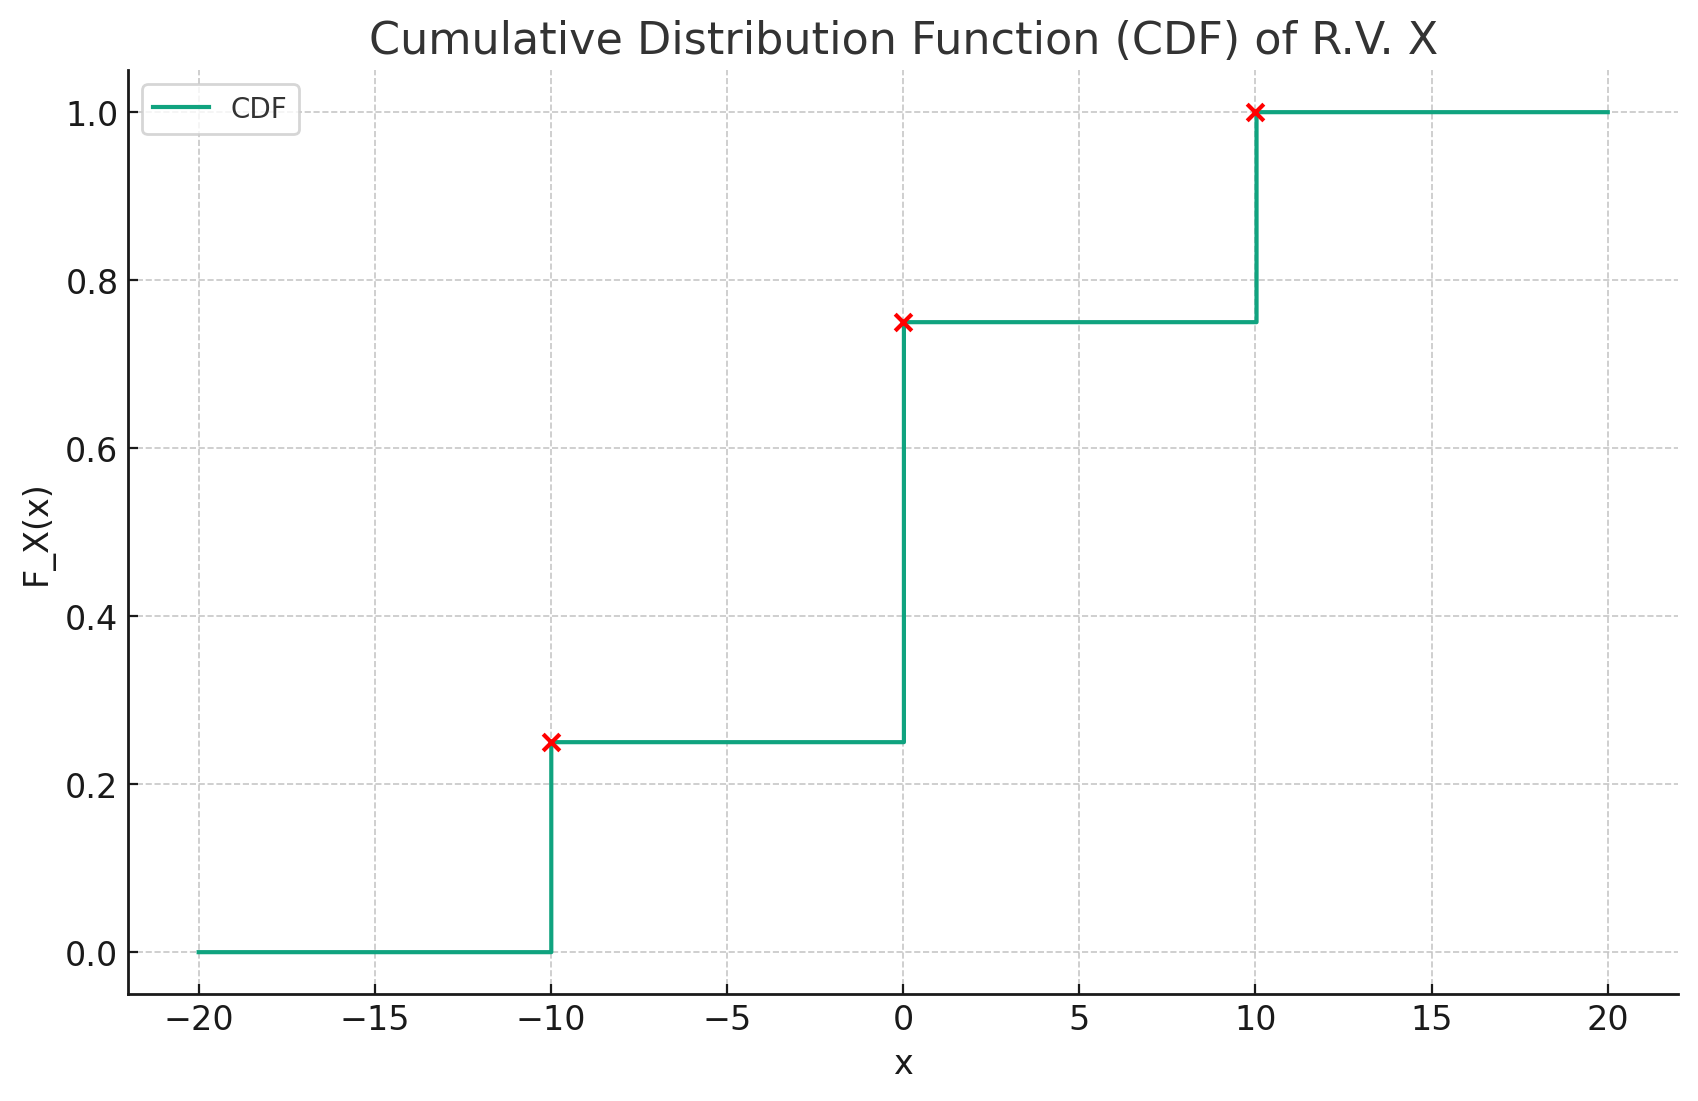
\includegraphics[width=0.7\textwidth]{cdf_plot.png}
\caption{Cumulative Distribution Function (CDF) of \( X \)}
\end{figure}
\newpage

\section*{Problem \#2 [10 pt]}
Consider a random process \( f(t) = A \cos(2\pi ft) \), where \( A \) is a Gaussian random variable with mean \( \mu_A = 5 \) and variance \( \sigma_A^2 = 2 \). We are tasked with finding the mean and power of \( f(t) \), its autocorrelation function, and determining if the process is wide-sense stationary (WSS).
\newline\newline
The mean of \( f(t) \) is given by:
\[ \mu_{f(t)} = E[A \cos(2\pi ft)] = \mu_A \cdot E[\cos(2\pi ft)] = 0 \]
\noindent
The power of \( f(t) \), denoted \( P_{f(t)} \), is:
\[ P_{f(t)} = E[f(t)^2] = (\sigma_A^2 + \mu_A^2) \cdot 0.5 = 13.5 \]
\noindent
The autocorrelation function \( R(\tau) \) is:
\[ R(\tau) = E[f(t)f(t + \tau)] = (\sigma_A^2 + \mu_A^2) \cdot \cos(2\pi f\tau) = 27 \cdot \cos(2\pi f\tau) \]
\noindent
The process is wide-sense stationary since the mean is constant and the autocorrelation function only depends on the time difference \( \tau \).
\newpage
\section*{Problem \#3 [10 pt]}

We aim to calculate the noise power in dBm for an 18 MHz IEEE 802.11ac Wi-Fi signal at a temperature of 300 K.
\newline\newline
The noise power can be calculated using Johnson-Nyquist noise formula:
\[ P = k \cdot T \cdot B \]
where:
\begin{itemize}
    \item \( P \) is the noise power in watts (W),
    \item \( k \) is the Boltzmann constant (\( 1.380649 \times 10^{-23} \) J/K),
    \item \( T \) is the absolute temperature in kelvins (K),
    \item \( B \) is the bandwidth in hertz (Hz).
\end{itemize}
\noindent
First, we convert the bandwidth from MHz to Hz:
\[ B = 18 \text{ MHz} = 18 \times 10^6 \text{ Hz} \]
\noindent
Then, we calculate the noise power in watts:
\[ P = (1.380649 \times 10^{-23}) \cdot 300 \cdot (18 \times 10^6) \]
\noindent
To convert the noise power from watts to dBm, we use the formula:
\[ P_{\text{dBm}} = 10 \cdot \log_{10}(P / 0.001) \]
\noindent
Upon calculation, the noise power in watts is approximately \( 7.456 \times 10^{-14} \) W, and when converted to dBm, it is approximately -101.28 dBm.
\newpage


\section*{Problem \#4 [20 pt]}
Consider a wide-sense stationary (WSS) random process \( M(t) \) with an autocorrelation function \( R_M(\tau) = \text{sinc}(5000\tau) \) serving as the message signal, where the maximum absolute value of the message signal \( m(t) \) is 1. Given a path loss of 100 dB and a noise spectral density \( N_0 = 10^{-12} \), the goal is to reach a signal-to-noise ratio (SNR) of 30 dB for various analog communication schemes. 

\noindent
The bandwidth for DSB-SC AM is twice the baseband bandwidth:
\[ B_{\text{DSB-SC AM}} = 2 \times B_{\text{baseband}} = 2 \times 5000 \text{ Hz} = 10000 \text{ Hz} \]
\newline
\noindent
The bandwidth for Conventional AM is the same as for DSB-SC AM:
\[ B_{\text{AM}} = B_{\text{DSB-SC AM}} = 10000 \text{ Hz} \]
\newline
\noindent
The bandwidth for FM using Carson's rule is:
\[ B_{\text{FM}} = 2 (\beta + 1) B_{\text{baseband}} = 2 (5 + 1) \times 5000 \text{ Hz} = 60000 \text{ Hz} \]
\newline
\noindent
The required transmitter power to achieve the desired SNR is calculated using the formula:
\[ P_{\text{TX}} = B \cdot N_0 \cdot 10^{\frac{\text{SNR}_{\text{dB}} + \text{Path Loss}}{10}} \]
where \( B \) is the bandwidth of the signal, \( N_0 \) is the noise spectral density, SNR in dB is the desired signal-to-noise ratio, and Path Loss is given in dB.
\noindent
\[ P_{\text{TX, DSB-SC AM}} = 10000 \text{ Hz} \times 10^{-12} \text{ W/Hz} \times 10^{\frac{30 + 100}{10}} = 100000 \text{ W} \]
\[ P_{\text{TX, DSB-SC AM}} \text{ in dBm} = 10 \cdot \log_{10}(100000 \text{ W} / 0.001) = 80 \text{ dBm} \]
\newline
\noindent
\[ P_{\text{TX, AM}} = P_{\text{TX, DSB-SC AM}} = 80 \text{ dBm} \]
\newline
\noindent
\[ P_{\text{TX, FM}} = 60000 \text{ Hz} \times 10^{-12} \text{ W/Hz} \times 10^{\frac{30 + 100}{10}} = 600000 \text{ W} \]
\[ P_{\text{TX, FM}} \text{ in dBm} = 10 \cdot \log_{10}(600000 \text{ W} / 0.001) \approx 87.78 \text{ dBm} \]
\noindent
The trade-offs among these communication schemes include bandwidth efficiency, power efficiency, and the complexity of the transmitter and receiver design. DSB-SC AM and Conventional AM require less bandwidth compared to FM but FM provides better noise immunity at the expense of increased bandwidth.
\newline
\begin{table}[h!]
\centering
\begin{tabular}{@{}lcc@{}}
\toprule
Modulation Scheme & Bandwidth (Hz) & TX Power (dBm) \\ \midrule
DSB-SC AM         & 10,000         & 80.00          \\
Conventional AM   & 10,000         & 80.00          \\
FM (\( \beta = 5 \)) & 60,000         & 87.78          \\ \bottomrule
\end{tabular}
\caption{Bandwidths and required transmitter powers for different analog communication schemes}
\end{table}

\newpage
\section*{Problem \#5 [10 pt]}
We are given a baseband signal on the in-phase branch of the IQ demodulator with a bandwidth of 9 MHz. The task is to determine an appropriate sampling rate (\( f_s \)) that includes a 1 MHz guard band to avoid aliasing during the sampling process.
\newline\newline
For a complex baseband signal, which includes both in-phase (I) and quadrature (Q) components, the minimum sampling rate to avoid aliasing is equal to the signal bandwidth. This is different from real signals, where the Nyquist theorem would require the sampling rate to be at least twice the bandwidth.
\newline\newline
To include a guard band of 1 MHz, we add this value to the signal's bandwidth to calculate the sampling rate:

\[ f_s = \text{Bandwidth} + \text{Guard Band} \]
\[ f_s = 9 \text{ MHz} + 1 \text{ MHz} \]
\[ f_s = 10 \text{ MHz} \]
\newline\newline
Thus, the sampling rate must be at least 10 MHz to ensure a guard band of 1 MHz and to avoid aliasing.
\newpage

\section*{Problem \#6 [10 pt]}
The task is to determine the appropriate sampling rates for a modulated signal with a bandwidth of 1 MHz around a carrier frequency of 915 MHz. We are considering two scenarios:
\begin{enumerate}
    \item Directly sampling the passband signal, which will require an RF ADC capable of handling high frequencies. The goal is to choose a sampling rate \( f_s \) that avoids aliasing.
    \item Using an IQ demodulator to represent the passband signal at baseband, which involves determining the sampling rates for the ADCs that will process the I and Q components.
\end{enumerate}
\noindent
For the passband signal, the Nyquist theorem dictates that the sampling rate must be at least twice the highest frequency present in the signal. The highest frequency is the sum of the carrier frequency and half of the signal's bandwidth. Therefore, the minimum sampling rate is calculated as:

\[ f_s \geq 2 \times (915 \text{ MHz} + 0.5 \text{ MHz}) \]
\[ f_s \geq 2 \times 915.5 \text{ MHz} \]
\[ f_s \geq 1831 \text{ MHz} \]
\noindent
For the I and Q components after IQ demodulation, each component must be sampled at least at the signal's bandwidth to avoid aliasing. Since the signal bandwidth is 1 MHz, the minimum sampling rate for both I and Q is:

\[ f_{s,I} = f_{s,Q} \geq 1 \text{ MHz} \]
\newpage

\newpage
\section*{Problem \#7 [10 pt]}

The task is to determine:
\begin{itemize}
    \item The number of discrete real samples needed to represent a modulated signal with a bandwidth of 1 MHz around a carrier frequency of 915 MHz, given that the time duration \( T \) is 10 milliseconds.
    \item The maximum time duration for which we can occupy the channel, assuming we are limited to using only 256 complex samples for representing the signal.
\end{itemize}

For a real signal with a 1 MHz bandwidth, the Nyquist sampling rate should be twice the bandwidth to avoid aliasing. Thus, for a 10 millisecond duration, the number of discrete real samples \( N \) required is calculated as follows:

\[ N = T \times f_{\text{Nyquist}} = 10 \times 10^{-3} \text{ s} \times 2 \times 1 \text{ MHz} = 20,000 \text{ samples} \]

Given the limitation of 256 complex samples, each complex sample can represent two real samples. The Nyquist rate for complex samples is equal to the bandwidth of the signal. The maximum channel occupation time \( T_{\text{max}} \) is therefore:

\[ T_{\text{max}} = \frac{\text{Number of real samples}}{f_{\text{Nyquist, complex}}} = \frac{512}{1 \text{ MHz}} = 512 \text{ microseconds} \]
\newpage
\section*{Problem \#8 [10 pt]}

The question is whether non-uniform quantization and uniform quantization can achieve the same performance when the amplitude of the signal being quantized follows a uniform distribution.
\newline\newline\newline
Uniform quantization divides the signal's range into intervals of equal size. If the signal amplitude is uniformly distributed, this is the optimal strategy because it minimizes the mean square quantization error.
\newline\newline
Non-uniform quantization, on the other hand, is designed for signal distributions with varying probabilities across the amplitude range. It is most efficient when the signal has higher probabilities in certain ranges, allowing for smaller intervals and hence, a lower quantization error in these regions.
\newline\newline
For a uniformly distributed signal, all amplitude ranges are equally probable. Therefore, non-uniform quantization does not provide an advantage, as it would not make sense to allocate more quantization levels to any particular amplitude range.



\newpage
\section*{Problem \#9 [10 pt]}
For a 3GPP 5G New Radio (NR) signal with a bandwidth of 400 MHz centered around a 28 GHz carrier, we are to determine:
\begin{itemize}
    \item The minimum ADC sample rates on the I- and Q- branches to ensure a 50 MHz guard band to prevent aliasing.
    \item The minimum noise power that the receiver observes in dBm for each branch at a temperature of 300° Kelvin.
\end{itemize}
\newline\newline
The signal in question has a complex structure, with both I (in-phase) and Q (quadrature) components. For such complex signals, the Nyquist rate is equal to the bandwidth. Considering the required 50 MHz guard band, the minimum ADC sample rate is calculated as:

\[ f_{s,min} = \text{Bandwidth} + \text{Guard Band} = 400 \text{ MHz} + 50 \text{ MHz} = 450 \text{ MHz} \]

\noindent
Thus, both I- and Q- branches should be sampled at a minimum rate of 450 MHz to avoid aliasing.
\newline\newline
The minimum noise power received is given by the thermal noise floor, which depends on the bandwidth and temperature. It can be calculated using the Boltzmann constant and is expressed in dBm. For a 400 MHz signal at 300° Kelvin, the noise power in dBm is given by:

\[ P_{\text{noise}} = k \cdot T \cdot B \]
\noindent
Where \( k \) is the Boltzmann constant (\( 1.380649 \times 10^{-23} \) J/K), \( T \) is the absolute temperature in kelvins, and \( B \) is the bandwidth in hertz. After calculating the noise power in watts, it is converted to dBm using the formula:

\[ P_{\text{noise,dBm}} = 10 \cdot \log_{10}\left(\frac{P_{\text{noise}}}{0.001}\right) \]
\noindent
The result is a minimum noise power of approximately -87.81 dBm for each branch.


\end{document}
